\documentclass[a4paper]{article}

\usepackage[brazilian]{babel}
\usepackage[utf8x]{inputenc}
\usepackage[T1]{fontenc}

\usepackage{float}

\usepackage{listings}
\usepackage{pythonhighlight}

%% Useful packages
\usepackage{amsmath}
\usepackage{graphicx}
\usepackage[colorinlistoftodos]{todonotes}
\usepackage[colorlinks=true, allcolors=blue]{hyperref}

\usepackage{mathrsfs}
\usepackage{amssymb}



%opening
\title{Relatório do Projeto 2}
\author{Daniel Moreira Cestari - 5746193}

\begin{document}

\maketitle

\section{Introdução}

O objetivo do Projeto 2 é o desenvolvimento de uma triangulação \textit{Delaunay} 2D. 

A definição de uma triangulação \textit{Delaunay} é uma triangulação de pontos tal que nenhum ponto do conjunto inicialmente fornecido está dentro do circuncirculo de qualquer triângulo da triangulação. Essa propriedade de nenhum ponto externo aos triângulos estar dentro do circuncirculo, garante que o mínimo ângulo dos triângulos será maximizado. É provado que dado um conjunto de pontos no espaço Euclidiano, a triangulação \textit{Delaunay} desses pontos é única, isso permite que a implementação deste trabalho possa ser testada utilizando outra biblioteca que já a implementa.

A entrada do algoritmo é um conjunto de pontos, e como saída o programa retorna na representação de uma \textit{Corner table} a triangulação \textit{Delaunay}  dos pontos passados.  O algoritmo para a triangulação empregado foi o algoritmo de inserção de pontos incrementalmente com \textit{flip} de arestas.

A estrutura de dados \textit{Corner table} foi implementada em atividade passadas da disciplina, mas até então possuía apenas operações de conjunta básica sobre os triângulos representados pela estrutura. Essas operações eram: fecho, estrela, anel, e \textit{link}. Para este trabalho foi necessário a inclusão de mais operações, como adição, remoção de triângulos, adição de vértices, busca de triângulos que compartilhem aresta, encontrar o triângulo que um dado ponto se encontra, coordenadas baricêntricas de um dado ponto, teste de orientação de pontos, teste do incirculo e \textit{flip} de arestas.



\section{Implementação}

Nesta seção é apresentada a implementação do código.

Abaixo é apresentado o esquema geral da implementação:
\begin{itemize}
	\item Determinação de um triângulo contendo os dados fornecidos (triângulo externo);
	
	\item Inserção incremental dos pontos fornecidos;
	\begin{itemize}
			\item Correção dos triângulos pelo teste do incírculo e \textit{flip} de arestas;
	\end{itemize}
	
	\item Remoção de todos os triângulos com vértices do triângulo externo;
	
	\item Limpeza da estrutura de dados de objetos eliminados.
	
\end{itemize}

Abaixo é exibida a função que calcula a triangulação:
%%%%%%%%%%%%%%%%%%%%
% def delaunay_triangulation
\inputpython{project2.py}{12}{182}
%%%%%%%%%%%%%%%%%%%%



A seguir, cada etapa será descrita com mais detalhes.

Na \textit{docstring} de cada método é apresentada uma descrição geral da função e de cada parâmetro.

\subsection{Determinação do triângulo externo}

Nesta etapa os pontos são centrado, é tomada a distância do ponto mais distante da origem como o raio de um círculo que engloba todos os pontos. Esse raio é definido como a coordenada $y$ do primeiro vértice do triângulo, a coordenada $x$ é definida como $0$. Para encontrar os outros dois pontos é feita uma rotação de $\frac{-2\pi}{3} rad$ do ponto inicial duas vezes. Por fim, aos pontos encontrados são levados para a localização inicial dos dados.

A figura \ref{fig:outer_triangle} ilustra esse processo.


\begin{figure}[H]
	\centering
	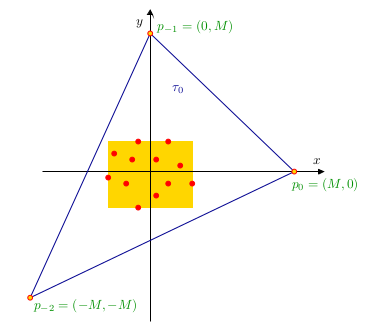
\includegraphics[width=.8\textwidth]{./imgs/outer_triangle.png}
	\label{fig:outer_triangle} 
	\caption[caption]{Exemplo de triângulo externo.}
\end{figure}



A seguir é mostrado a função que calcula os vértices do triângulo externo.
%%%%%%%%%%%%%%%%%%%%
% def outer_triangle
\inputpython{project2.py}{223}{254}
%%%%%%%%%%%%%%%%%%%%




\subsection{Encontrar triângulo que contém determinado ponto}

Esta função retorna o índice do triângulo que contém o ponto passado. Basicamente é feita uma busca aleatória dos triângulos presentes na estrutura de dados. Através das coordenadas baricêntricas é possível determinar se o ponto pertence ao triângulo em questão.

Posteriormente o Professor passou um algoritmo para a determinação de tal triângulo, mas este algoritmo ainda não foi implementado.




%%%%%%%%%%%%%%%%%%%%
% def find_triangle
\inputpython{corner_table.py}{304}{386}
%%%%%%%%%%%%%%%%%%%%


\subsection{Encontrar triângulos que compartilhem aresta}

Esta função permite fazer a busca pelos índices dos \textit{corners} ou pelas arestas. As arestas são definidas pelos índices dos vértices, sem importar a ordem dos vértices. É retornado o índice dos dois triângulos que compartilhem a aresta passada.

Para essa busca, os vértices são convertidos nos seus respectivos \textit{corners}, então é feita uma simples consulta a estrutura de dados para pegar a primeira face, e a segunda faces é determinada pelo \textit{corner} à direita do primeiro.

A figura \ref{fig:find_triangle} ilustra um exemplo. É passada a aresta $(V2,V3)$, são determinados os \textit{corners} relacionados à esses vértices, no caso ${C_2, C_3, C_4, C_5}$. Como os \textit{corners} são armazenados na estrutura orientados, é preciso apenas do primeiro \textit{corner} relacionado à $V2$, e com o \textit{corner} à direita desse já consegue-se determinar o triângulo adjacente.
 

\begin{figure}[H]
	\centering
	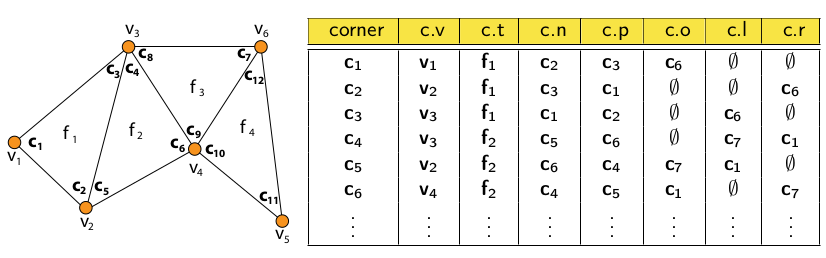
\includegraphics[width=1.0\textwidth]{./imgs/corner_table_example.png}
	\label{fig:find_triangle} 
	\caption[caption]{Exemplo de \textit{Corner table}.}
\end{figure}


A seguir é exibida o código da função que encontra os triângulos que compartilham aresta.
%%%%%%%%%%%%%%%%%%%%
% def triangles_share_edges
\inputpython{corner_table.py}{248}{289}
%%%%%%%%%%%%%%%%%%%%



\subsection{Remover triângulo}

Função bem simples, que por questões de eficiência apenas marca as linhas dos \textit{corners} do triângulo como $-1$ sem remover os elementos da \textit{Corner table}. Como, também por questões de eficiência na busca, são mantidas estruturas \textit{hash} auxiliares para relacionar um dado vértice a seus \textit{corners} e uma dada face a seus \textit{corners}, essas estruturas precisam ser atualizadas. Por fim é reatribuído os \textit{corners} à direita e esquerda e \textit{corners} opostos, dos \textit{corners} que faziam referência aos \textit{corners} removidos, basicamente as faces que compartilhavam arestas.


A seguir é exibida o código da função que remove triângulos.
%%%%%%%%%%%%%%%%%%%%
% def remove_triangle
\inputpython{corner_table.py}{545}{594}
%%%%%%%%%%%%%%%%%%%%




\subsection{Adicionar triângulo}

Operação simples de adicionar um triângulo especificado por 3 vértices. Primeiro verifica se a ordem dos vértices passados segue a orientação da estrutura, se não inverte a ordem, depois são adicionados os vértices nas estruturas auxiliares, por fim 3 \textit{corners} representando o triângulo são adicionados à \textit{Corner table}. Um último passo é recalcular os \textit{corners} à direita, esquerda e opostos dos \textit{corners} inseridos e dos restantes.


A seguir é exibida o código da função que adiciona triângulos.
%%%%%%%%%%%%%%%%%%%%
% def add_triangle
\inputpython{corner_table.py}{597}{681}
%%%%%%%%%%%%%%%%%%%%



\subsection{Legalização de triângulos}

Está é uma função importante que garante que quando um ponto é inserido na triangulação já existente, os triângulos modificados continuem sendo \textit{Delaunay}.

É passado para a função um ponto, o ponto que foi inserido, e a face desse ponto. É verificado então se o vértice oposto ao ponto inserido, com relação à aresta oposta, respeita o teste do incírculo, caso o vértice oposto esteja dentro do circuncirculo do triângulo adicionado, é realizado o \textit{flip} da aresta. Esse \textit{flip} resulta em dois outros triângulos que novamente precisam ser verificados em relação ao mesmo ponto e suas arestas opostas.


A figura \ref{fig:flip} ilustra um exemplo de \textit{flip} de aresta realizado durante a legalização.


\begin{figure}[H]
	\centering
	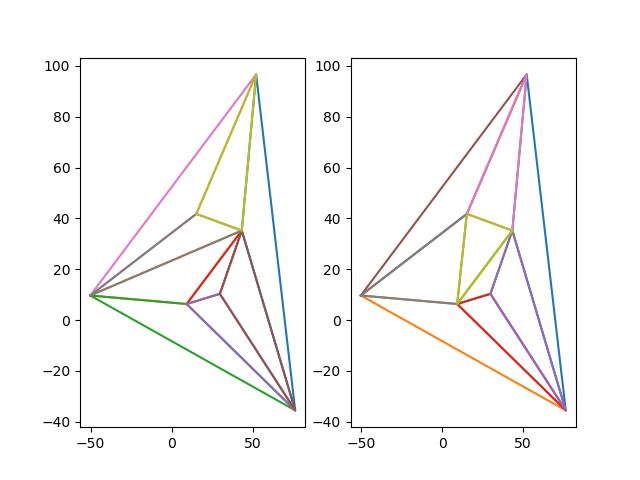
\includegraphics[width=1.0\textwidth]{./imgs/flip_example.png}
	\label{fig:flip} 
	\caption[caption]{Exemplo de \textit{flip} de aresta.}
\end{figure}

A seguir é exibida o código da função que legaliza arestas.
%%%%%%%%%%%%%%%%%%%%
% def legalize
\inputpython{corner_table.py}{163}{244}
%%%%%%%%%%%%%%%%%%%%


A operação de \textit{flip} é bem simples, dados dois triângulos que compartilhem uma aresta, esta aresta que eles compartilham é trocada pela aresta dos vértices opostos. Na implementação isso é feito removendo-se os dois triângulos e adicionando dois outros. 

A seguir é exibida o código da função que faz \textit{flip} de arestas.
%%%%%%%%%%%%%%%%%%%%
% def flip_triangles
\inputpython{corner_table.py}{468}{541}
%%%%%%%%%%%%%%%%%%%%





\subsection{Limpeza da estrutura}

Esta função é chamada após a triangulação ser concluída para remover os \textit{corners} excluídos da estrutura. Basicamente recalcula os índices dos \textit{corners}, vértices e faces, e agora sim removendo as entradas excluídas.


A seguir é exibida o código da função que limpa a estrutura.
%%%%%%%%%%%%%%%%%%%%
% def _clean_table
\inputpython{corner_table.py}{53}{111}
%%%%%%%%%%%%%%%%%%%%


\subsection{Outras funções}

Os métodos descritos anteriormente são os principais para a triangulação, no entanto, a fim de validar a implementação outras funções foram implementadas.

\begin{itemize}	
	\item \textbf{\textit{plot}:} Esta função faz o \textit{plot} da triangulação obtida;
	\item \textbf{\textit{test\_delaunay}:} Faz a contagem do número de faces, de faces orientadas e de faces \textit{delaunay};
	\item \textbf{\textit{bari\_coord}:} Calcula as coordenada baricêntricas de um ponto;
	\item \textbf{\textit{inCircle}:} Realiza o teste do incirculo;
	\item \textbf{\textit{orientation}:} Verifica se a orientação de 3 pontos está consistente;
	\item \textbf{\textit{fix\_opposite\_left\_right}:} Calcula os \textit{corners} opostos, à direita e esquerda, mantendo a estrutura consistente.
\end{itemize}



\section{Resultados}


Nesta seção são apresentados os resultados da implementação.


Alterando os parâmetros \textit{plot}, \textit{legalize} e \textit{legalize\_plot} da função que realiza a triangulação, as figuras \ref{fig:ex2_final} e \ref{fig:ex3_final} foram obtidas. Esses parâmetros permitem fazer \textit{plots} da triangulação passo a passo.

A figura \ref{fig:ex2_final} Mostra a inserção de pontos, no triângulo externo, sem o processo de legalização das arestas. Com isso é possível ver como a simples adição de pontos pode resultar em triângulos alongados, de qualidade ruim. 


\begin{figure}[H]
	\centering
	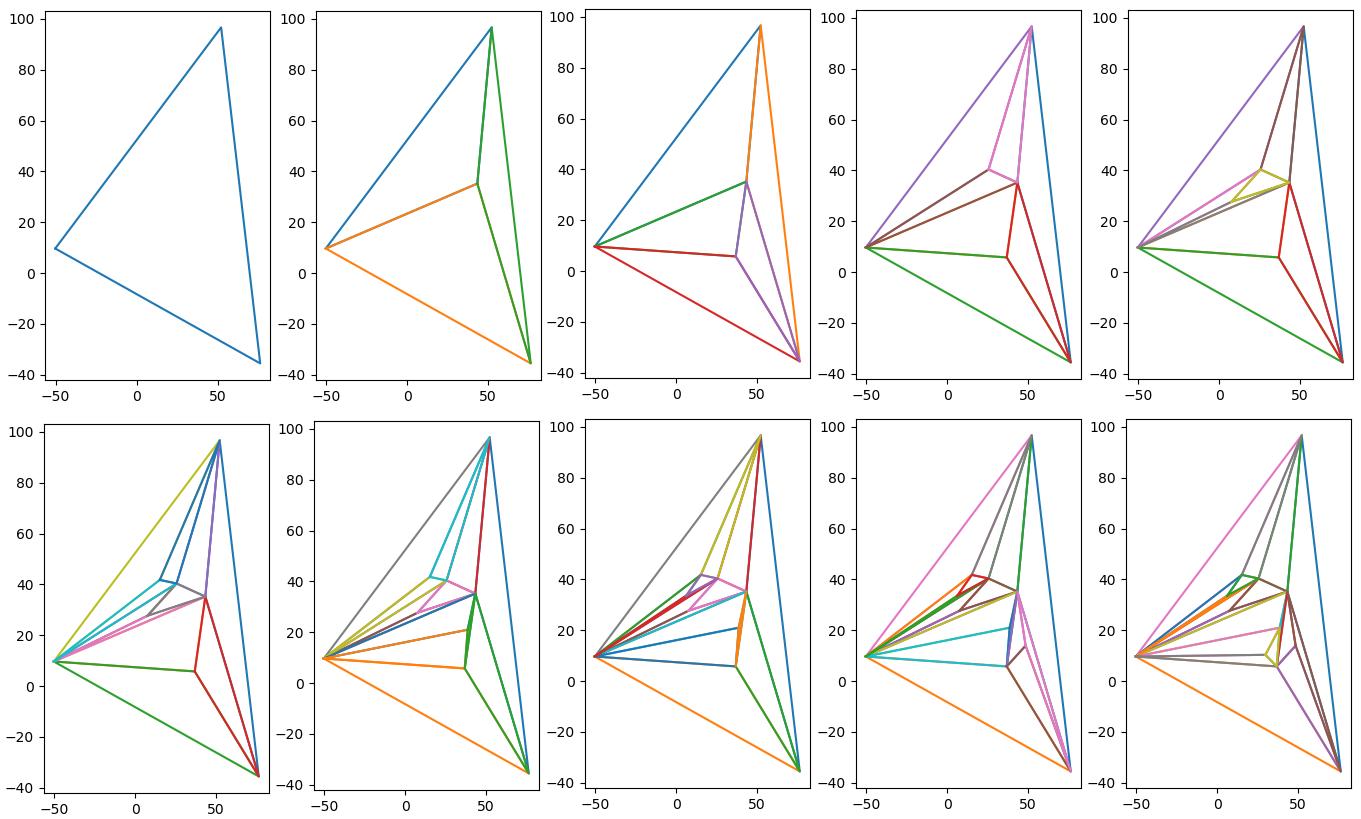
\includegraphics[width=1.0\textwidth]{./imgs/ex2_final.png}
	\label{fig:ex2_final} 
	\caption[caption]{Passo a passo da inserção de pontos \textbf{sem} legalização de arestas.}
\end{figure}

Já na figura \ref{fig:ex3_final} é exibida a inserção dos mesmos pontos, embora que em ordem diferente já que inserção dos pontos é aleatória, mas agora com a legalização das arestas. Isso garante que a cada inserção a triangulação continue sendo \textit{Delaunay}.

\begin{figure}[H]
	\centering
	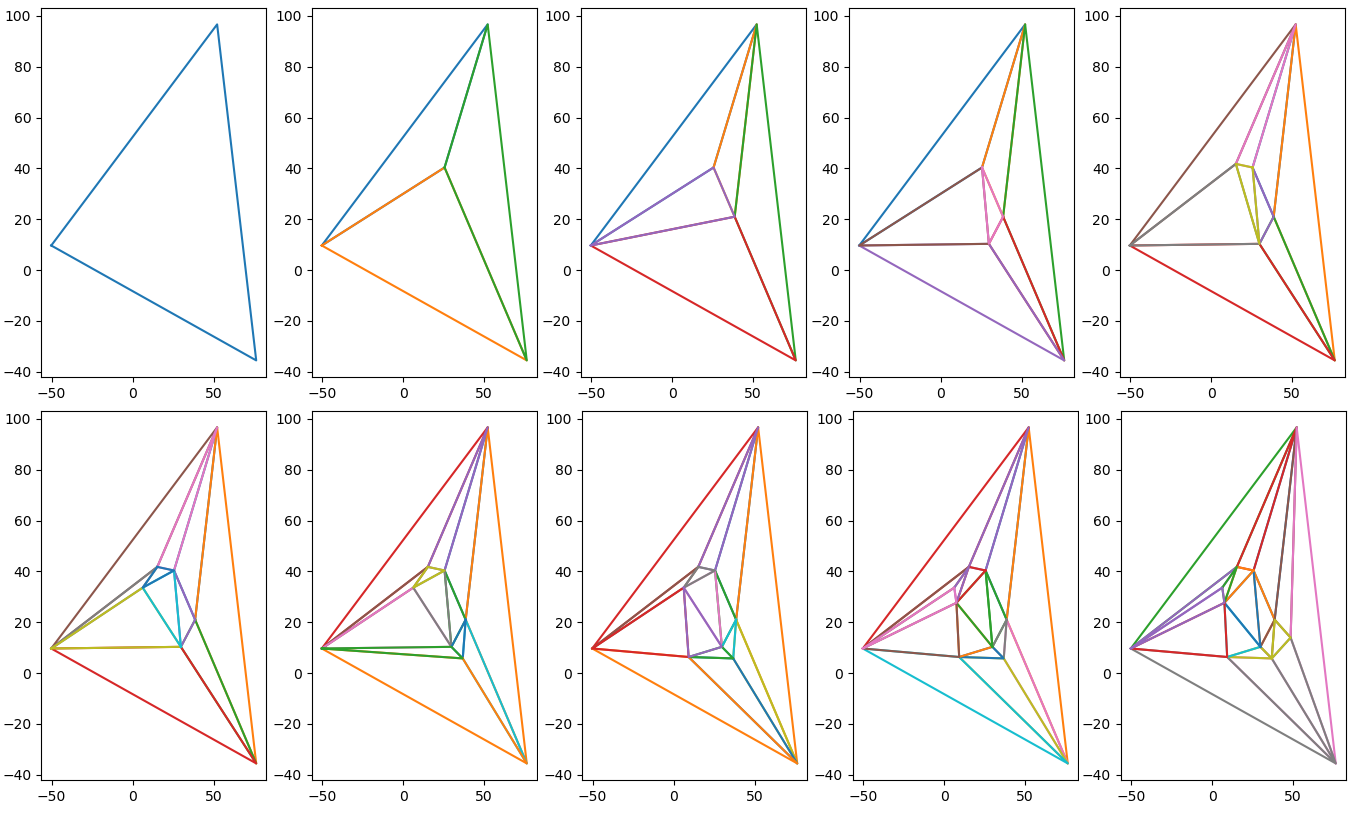
\includegraphics[width=1.0\textwidth]{./imgs/ex3_final.png}
	\label{fig:ex3_final} 
	\caption[caption]{Passo a passo da inserção de pontos \textbf{com} legalização de arestas.}
\end{figure}



A seguir é exibido um exemplo de código para execução de uma triangulação \textit{Delaunay} de 50 pontos gerados aleatoriamente segundo uma distribuição uniforme de 0 a 50. A figura \ref{fig:ex1} mostra o resultado final da triangulação, à direita é exibida a triangulação obtida pela bibliteca \textit{SciPy}, em azul, e à direita a triangulação obtida pela implementação do projeto. Neste exemplo, o triângulo externo ainda não foi removido. A figura \ref{fig:ex1_not_convex} mostra a triangulação com a remoção do triângulo externo.



\begin{verbatim}
# example with random points
import imp
import project2 as pjt
import corner_table as cnt
from scipy.spatial import Delaunay
import matplotlib.pyplot as plt
from numpy.random import uniform
from numpy import array, matrix, vstack, ndarray


# generate the random points with the outer triangle englobing them
low, high, size = 0, 50, 10
rd_pts = ndarray(buffer=uniform(low=low, high=high, size=2*size), 
								dtype=float, shape=(size, 2))
outer_pts = pjt.outer_triangle(rd_pts)
rd_pts = vstack((outer_pts, rd_pts))


grd_truth = Delaunay(points=rd_pts, furthest_site=False, incremental=True)
my_delaunay = pjt.delaunay_triangulation([tuple(i) for i in rd_pts[3:]])

plt.subplot(1,2,1)
plt.triplot(rd_pts[:,0], rd_pts[:,1], grd_truth.simplices.copy())
edges = my_delaunay.plot(show=True, subplot={'nrows':1, 'ncols':2, 'num':2})

plt.close('all')

grd_table = cnt.CornerTable()
a = [grd_table.add_triangle([tuple(i) for i in rd_pts[t]]) 
						for t in grd_truth.simplices]
my_delaunay.test_delaunay()
grd_table.test_delaunay()

\end{verbatim}



\begin{figure}[H]
	\centering
	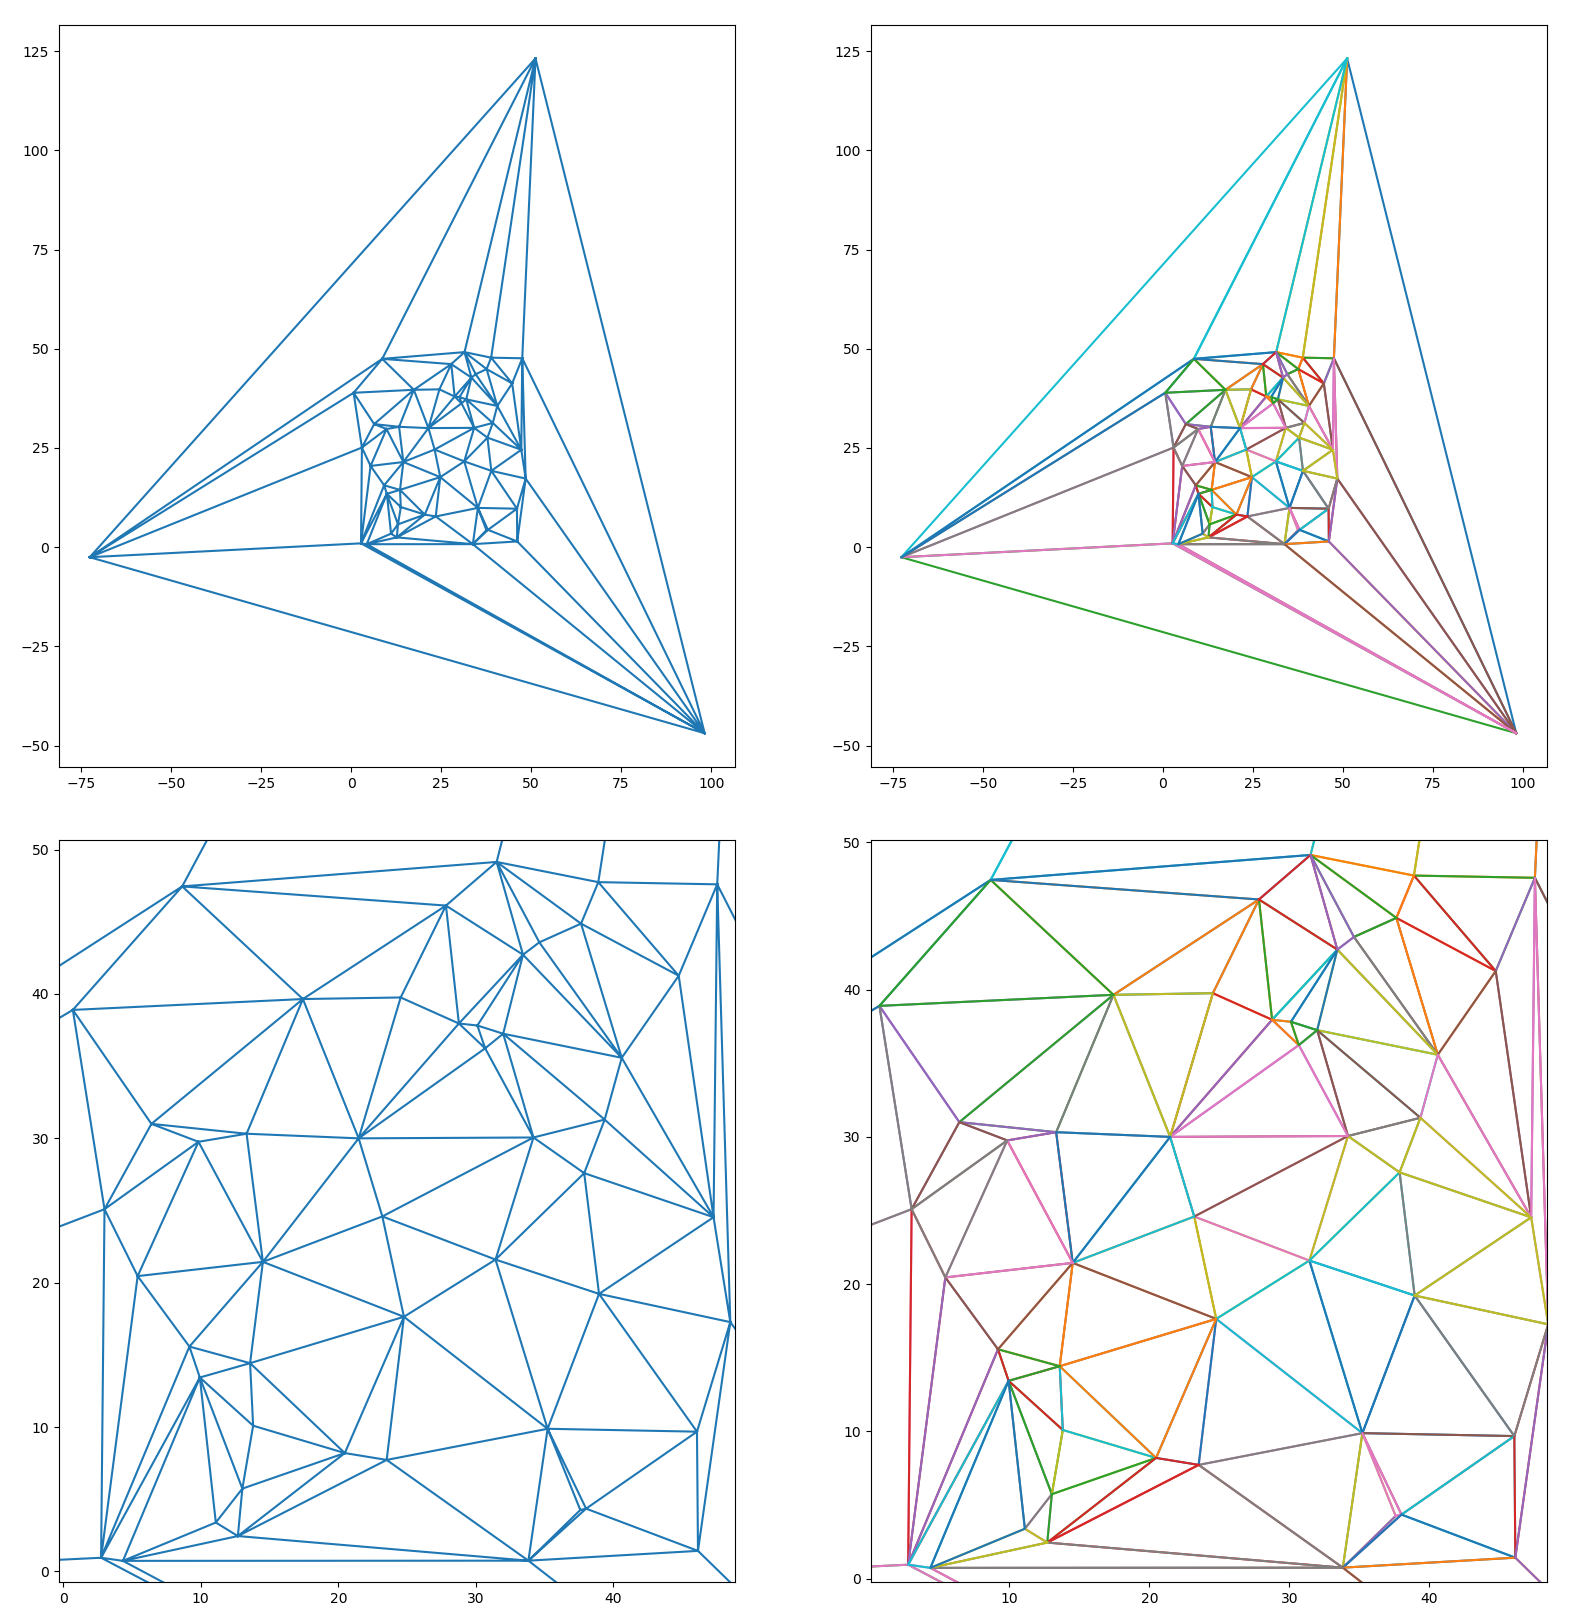
\includegraphics[width=1.0\textwidth]{./imgs/ex1_outer.png}
	\label{fig:ex1} 
	\caption[caption]{Exemplo de triangulação com 50 pontos aleatórios, ainda com o triângulo externo. Triangulação à esquerda gerada pela biblioteca \textit{SciPy}, à direita gerada pela implementação do projeto. Na parte de baixo é exibida a versão ampliada na triangulação.Triangulação à esquerda gerada pela biblioteca \textit{SciPy}, à direita gerada pela implementação do projeto.}
\end{figure}

Um detalhe importante no exemplo da figura \ref{fig:ex1_not_convex} é que nas referência do algoritmo de inserção de pontos incremental, não há referência sobre a inserção do fecho convexo ao final da triangulação. E o exemplo da figura deixa claro que em alguns casos, quando os vértices, e por consequência os triângulos, do triângulo externo são removidos, a triangulação resultante pode não ser convexa. Apesar disso a biblioteca \textit{SciPy} corretamente resulta numa triangulação que é convexa. E pelo exemplo anterior, figura \ref{fig:ex1}, fica claro que se ambas as triangulações deixarem o triângulo externo, o resultado é o mesmo, então a diferença está no passo após a remoção do triângulo externo.


\begin{figure}[H]
	\centering
	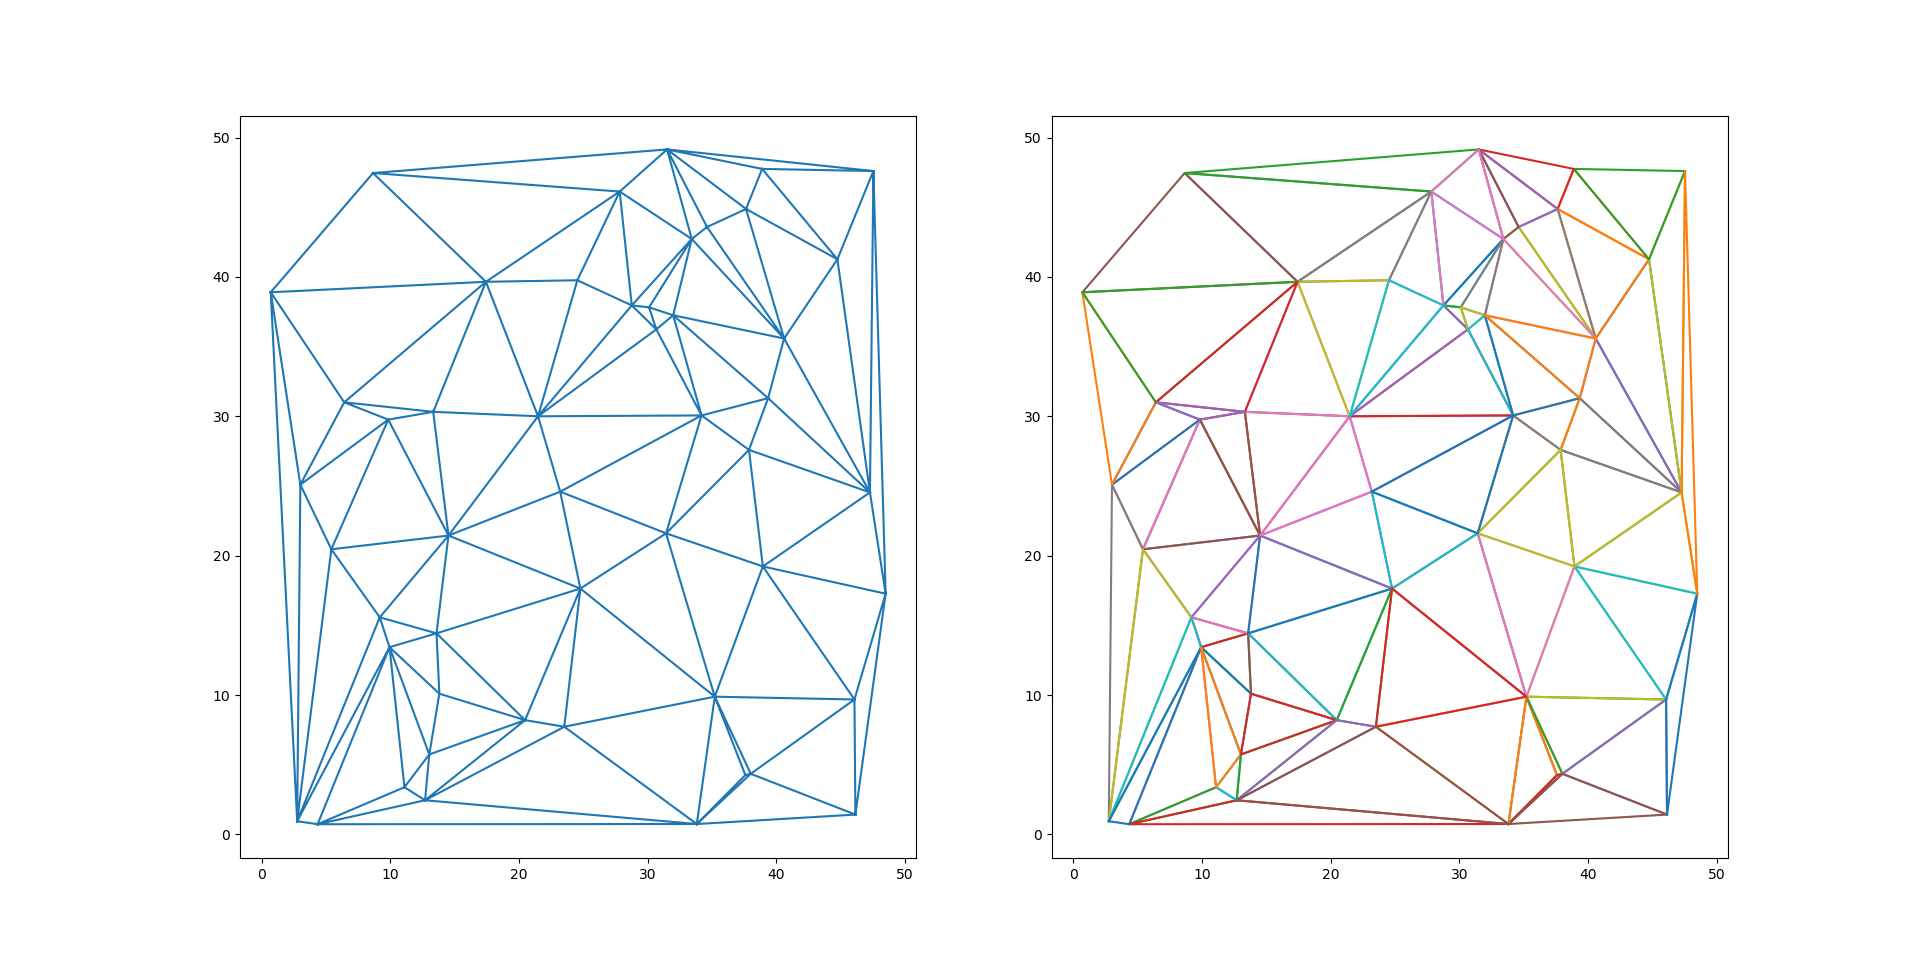
\includegraphics[width=1.0\textwidth]{./imgs/ex1_not_convex.png}
	\label{fig:ex1_not_convex} 
	\caption[caption]{Exemplo de triangulação final com 50 pontos aleatórios. Detalhe para a diferença entre as triangulações, a da direita convexa e a da esquerda não convexa. Triangulação à esquerda gerada pela biblioteca \textit{SciPy}, à direita gerada pela implementação do projeto.}
\end{figure}





%
%\subsection{Aerofólio}
%
%Código para gerar uma malha para a curva \textit{naca012}, a resolução da malha é determinada pela quantidade de pontos na curva. O domínio com comprimento 4, altura 6, e comprimento 1 à direita da curva. O domínio é divido em 4 partes, e o refinamento é feito ao redor da curva e após a curva no centro do domínio em relação à \textit{y}, ou $\eta$.
%
%
%Código utilizando a heurística 1.
%\begin{verbatim}
%imp.reload(pjt);  
%grid = pjt.generate_grid(filename_curve="naca012.txt", 
%left_border=1, domain_length=4, domain_height=3,
%heuristic=pjt.heuristic_1, k=3, filename_borders="naca012_h1", 
%xis_rf0=[1], xis_rf1=[0], etas_rf1=[0.419], a_xis0=[5], 
%a_xis1=[2.5], c_xis0=[5], c_xis1=[5], a_etas1=[5], c_etas1=[15])
%\end{verbatim}
%
%Código utilizando a heurística 2.
%\begin{verbatim}
%imp.reload(pjt);  
%grid = pjt.generate_grid(filename_curve="naca012.txt", 
%left_border=1, domain_length=4, domain_height=3,
%heuristic=pjt.heuristic_2, k=3, filename_borders="naca_h2", 
%xis_rf0=[1], xis_rf1=[0], etas_rf1=[0.419], a_xis0=[5], 
%a_xis1=[2.5], c_xis0=[5], c_xis1=[5], a_etas1=[5], c_etas1=[15])
%\end{verbatim}
%
%
%\begin{figure}[H]
%	\centering
%	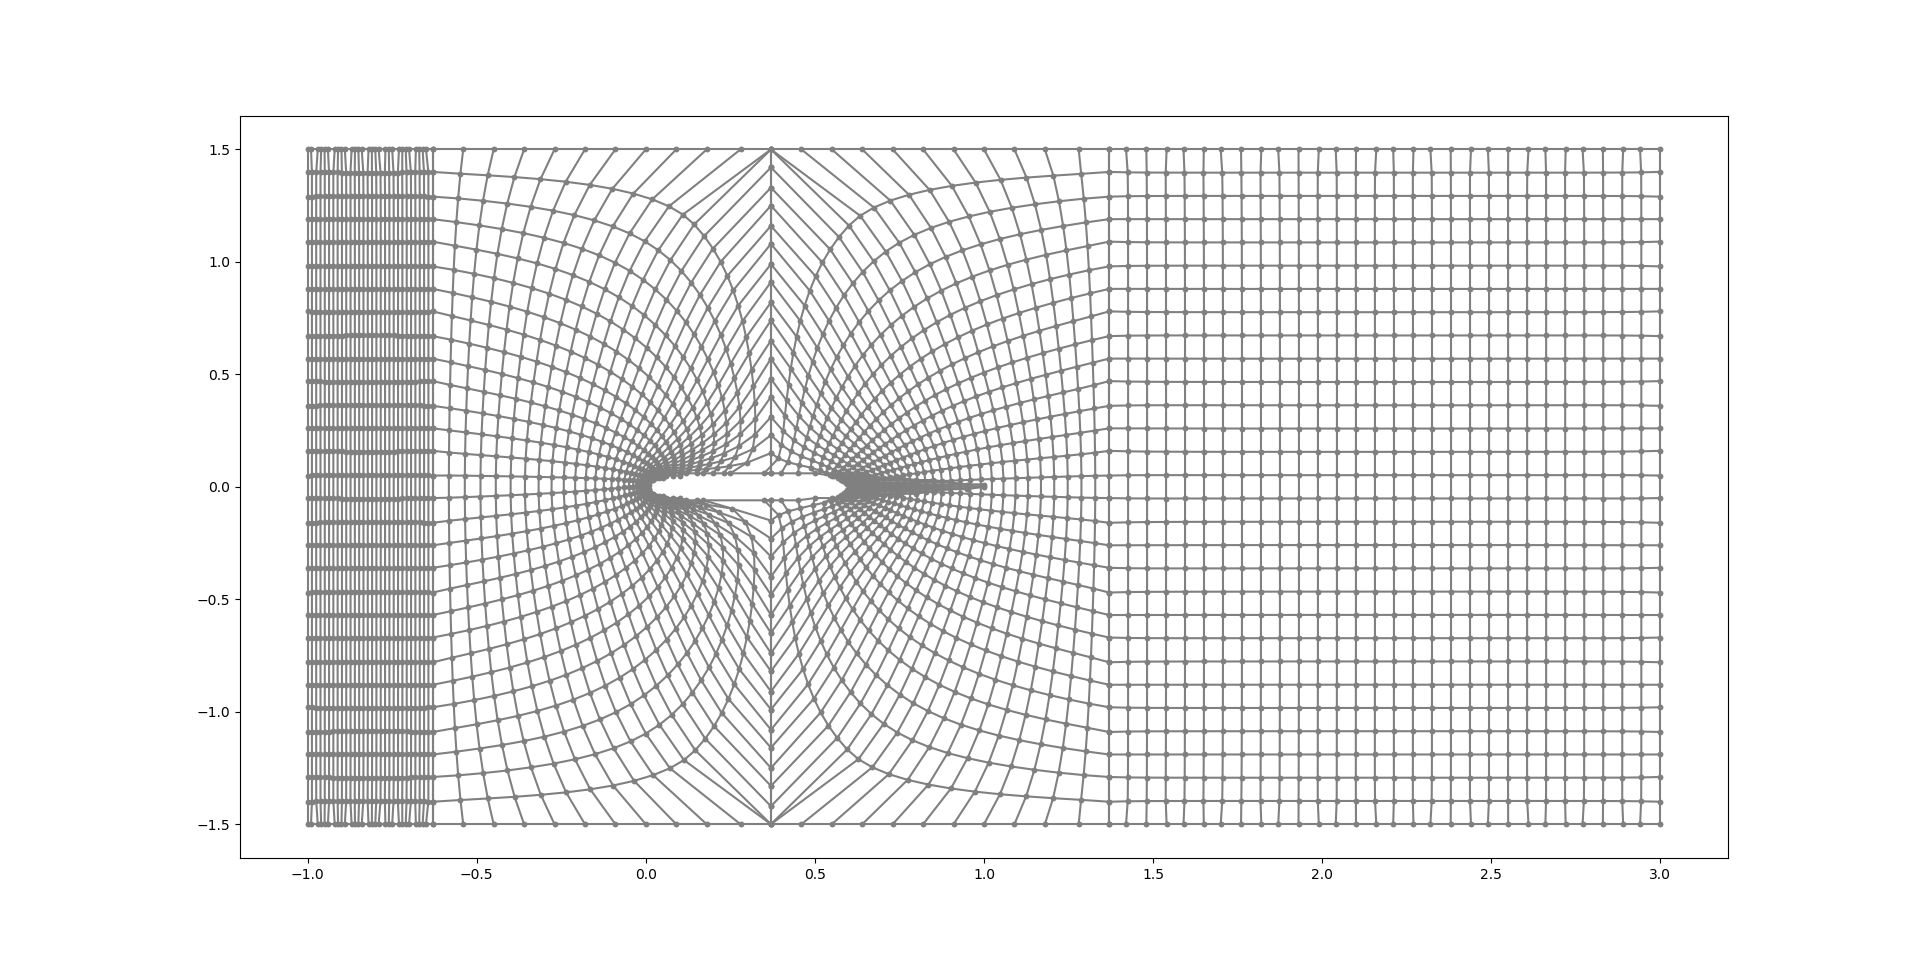
\includegraphics[width=1.0\textwidth]{naca_h1.png}
%	\label{fig:naca_h1} 
%	\caption[caption]{Malha gerada para a curva \textit{naca012 } pela heurística 1 sem refinamento.}
%\end{figure}
%
%\begin{figure}[H]
%	\centering
%	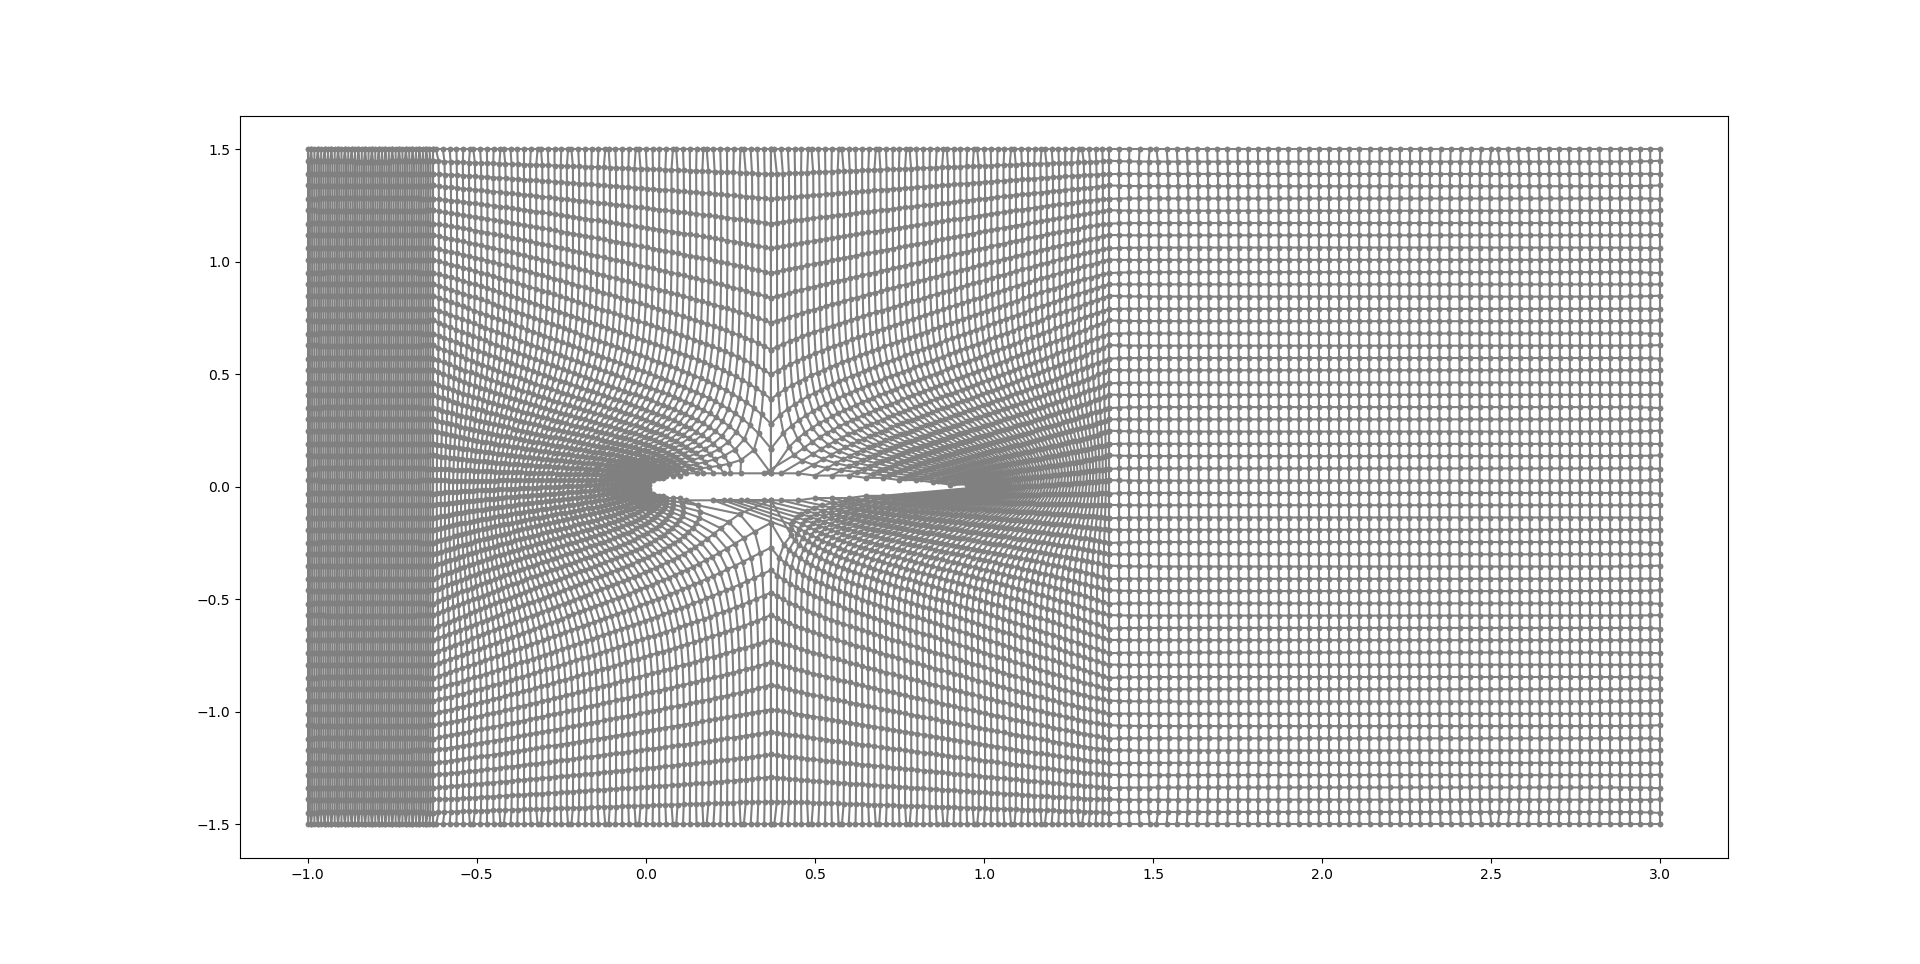
\includegraphics[width=1.0\textwidth]{naca_h2.png}
%	\label{fig:naca_h2} 
%	\caption[caption]{Malha gerada para a curva \textit{naca012 } pela heurística 2 sem refinamento.}
%\end{figure}
%
%
%
%\begin{figure}[H]
%	\centering
%	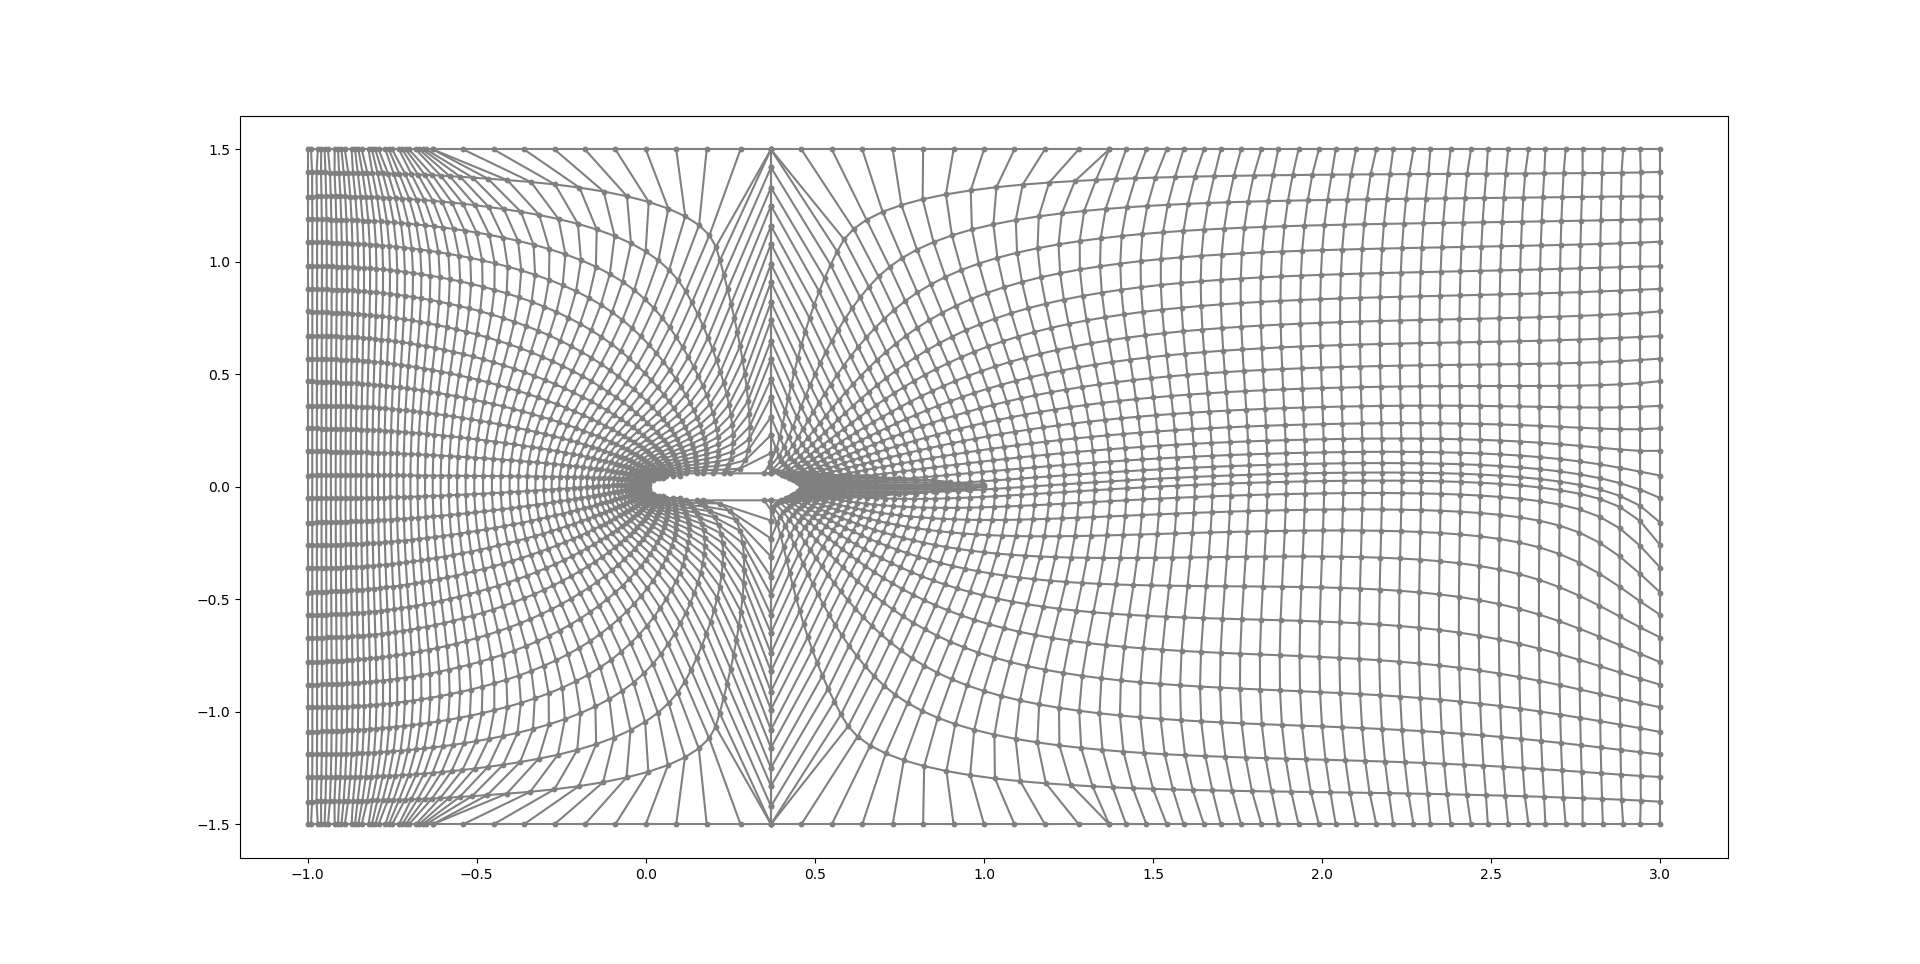
\includegraphics[width=1.0\textwidth]{naca_h1_refined.png}
%	\label{fig:naca_h1_refined} 
%	\caption[caption]{Malha gerada para a curva \textit{naca012 } pela heurística 1 com refinamento.}
%\end{figure}
%
%\begin{figure}[H]
%	\centering
%	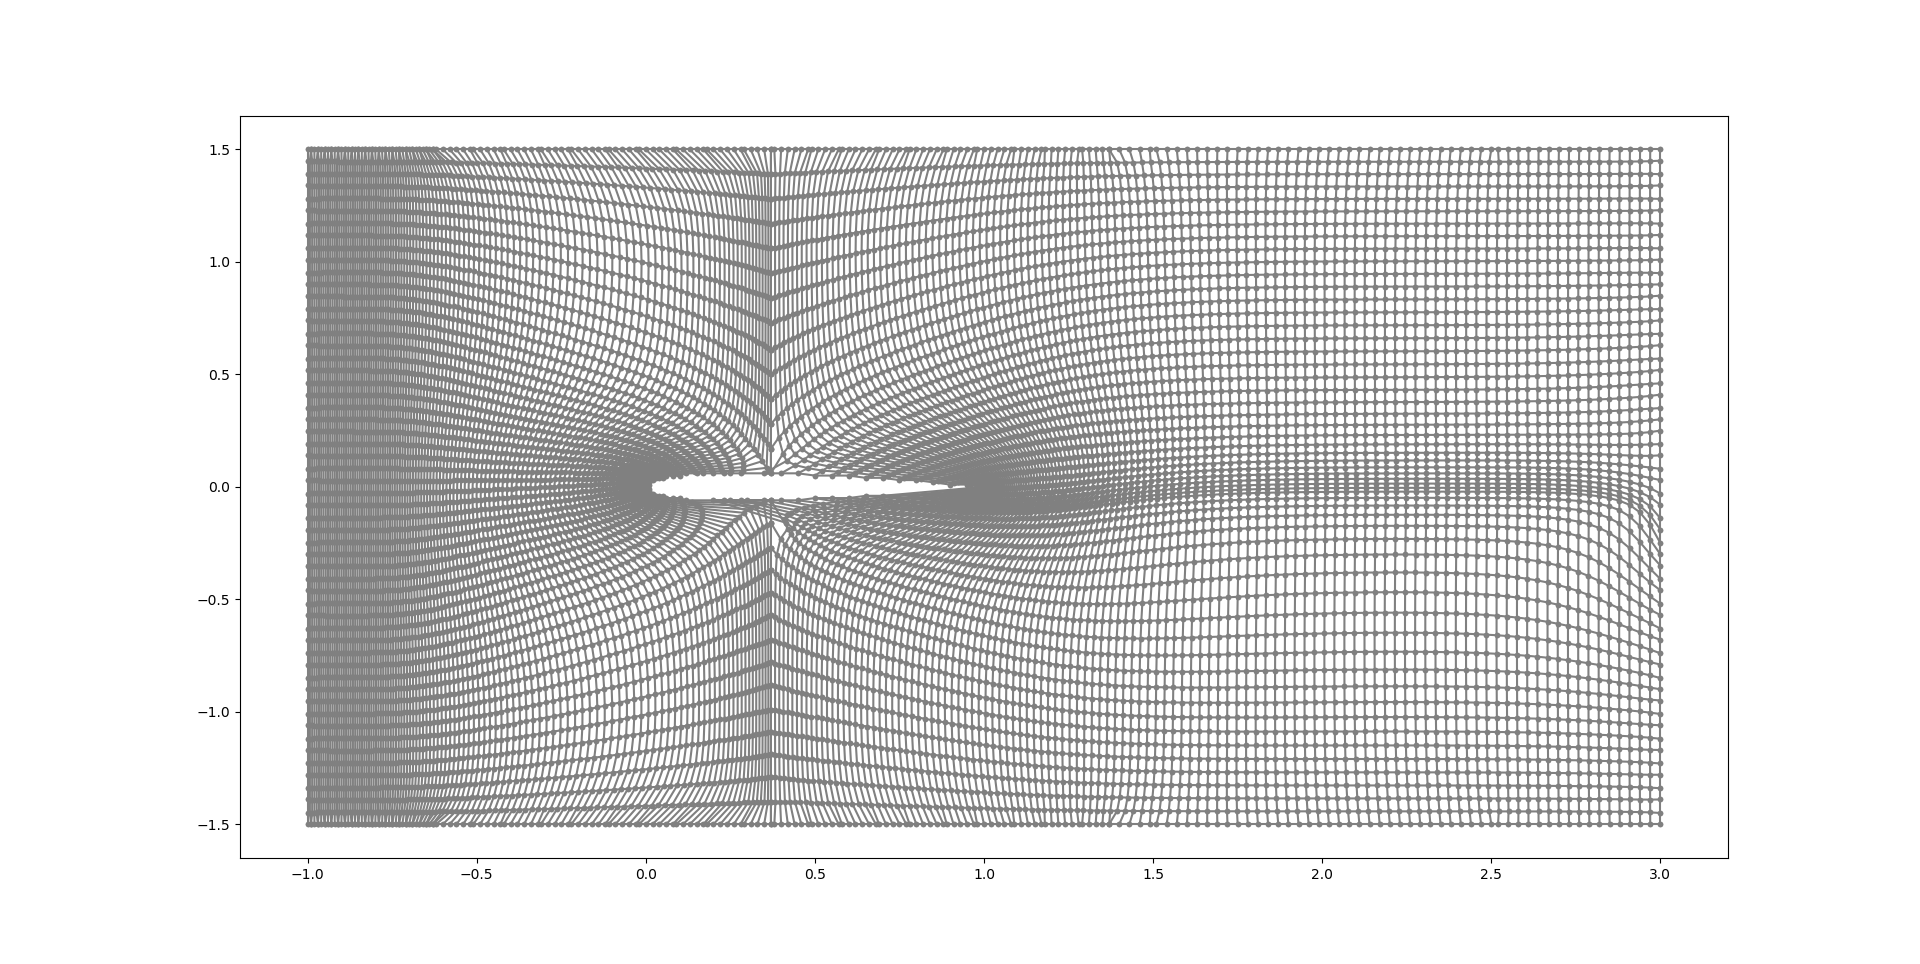
\includegraphics[width=1.0\textwidth]{naca_h2_refined.png}
%	\label{fig:naca_h2_refined} 
%	\caption[caption]{Malha gerada para a curva \textit{naca012 } pela heurística 2 com refinamento.}
%\end{figure}





\end{document}
